


\section{Scientific background}

    \subsection{Breast Cancer Overview}
   
    Breast cancer is the leading cause of cancer-related deaths among women in developed countries \cite{ferlay2015cancer}. It has been estimated that approximately 2.4 million females developed breast cancer in 2015, and it was the cause of death for more than 520,000 individuals \cite{Fitzmaurice2017Global2015}.  Denmark has the second highest disease incidence rate per 100,000 individuals in the world \cite{2015BreastInternational}. 
    
    Screening programs, education, and improved therapeutic strategies have decreased the mortality rates from this disease, but not at the desired magnitude. The most plausible explanation for this discordance is the lack of a complete picture of the biologic heterogeneity of breast cancers \cite{Vidal2017}.
    Breast cancer is not a single disease, but is composed of multiple subtypes with distinct morphologies and clinical implications \cite{Dai2015}. Growing evidence implies that carcinomas with different histopathological and biological features exhibit distinct behaviours that lead to different treatment responses and require tailored therapeutic approaches \cite{Blows2010}. Therefore, accurate grouping of breast cancers into clinically relevant subtypes is of high importance for prognosis prediction and treatment decision making.

    \subsection{Disease Management and Prognosis}
    
    Historically, prognostication in breast cancer has relied on the clinicopathological parameters such as patient age, tumour size, lymph node involvement, presence of metastasis, histological grade, and individual molecular markers such as hormone receptors, human epidermal growth factor status (HER2), and proliferation marker Ki67. All of these are routinely used in clinics to stratify patients for prognostic predictions, to assign treatments, and to include patients into clinical trials \cite{Vidal2017}.

    The limitations of these markers in predicting risk of recurrence has led to the use of mRNA- and DNA-based markers. The advent of high-throughput platforms for gene expression profiling has shown that tumour cell response to treatment is not determined by anatomical prognostic factors but rather intrinsic molecular characteristics \cite{Iwamoto2010PredictingData}. The large-scale analysis of the genetic makeup of tumours has permitted understanding of the genomic and transcriptomic landscape of breast cancer. It has brought the concept of breast cancer heterogeneity to the forefront of cancer research, and the fact that distinct subtypes of breast cancer are completely different diseases that affect the same anatomical site \cite{weigelt2010}. This new strategy has changed how breast cancer patients are managed and treated, which provided an incremental increase on the reproducibility and accuracy of disease prognosis and therapy selection \cite{pusztai2008}. Importantly, though, the prognostic and predictive power of molecular profiling has been shown to be complementary to, rather than a replacement for, traditional clinicopathological parameters \cite{weigelt2010}.

   
    \subsection{Classification Conventions}
    
    Breast cancers can be classified by different schemata. Each of these aspects influences treatment response and prognosis.  This section will present the main traditional and novel breast cancer classification conventions to introduce the overwhelming heterogeneity observed among the patients. 
    %[more about heterogeneity?]

    \subsubsection{Cancer Staging by TNM}
    
    Cancer staging is a way of determining and describing cancer location and spread in the body. The underlying purpose of staging is to characterise the extent or severity of an individual’s cancer, and to bring together cancers that have similar prognosis and treatment \cite{2017AJCCStaging}. 

    Breast cancer is staged using the TNM system developed by The American Joint Committee on Cancer (AJCC) and the International Union Against Cancer (UICC) \cite{Giuliano2017}. The TNM staging system is the most common tool used by clinicians to converge the results from diagnostic tests and scans, and it involves two steps. Firstly, cancer is classified by several factors, \textbf{T} for the extent of the tumour, \textbf{N} for the extent of spread to the nodes, and \textbf{M} for the presence of metastasis. Then, these are grouped as TNM factors to find the overall cancer stage. Table \ref{table:tnmstage} shows the overview of TNM combinations. There are 5 stages: stage 0 (zero), which is noninvasive \textit{in situ} carcinoma, and stages I through IV (1 through 4), which are used for invasive breast cancer.


    % TNM TABLE
        \begin{table}[!h]
        \centering
        \tiny
        \caption{AJCC/UICC TNM anatomic cancer staging and prognostic groups reference table.  The combination of T, N, and M is used to assign the  overall stage (substage).}
        \label{table:tnmstage}
        \begin{tabular}{c|c|c|c|c}
        \multicolumn{2}{c|}{\textbf{\small Stage}} & \textbf{Tumour} & \textbf{Nodes} & \textbf{Metastasis} \\ \hline
        \textbf{0} & 0 & Tis & N0 & M0 \\ \hline
        \textbf{1} & IA & T1 & N0 & M0 \\ \hline
        \textbf{} & IB & T0 & N1mi & M0 \\ \cline{2-5} 
        \textbf{} &  & T1 & N1mi & M0 \\ \hline
        \textbf{2} & IIA & T0 & N1 & M0 \\ \hline
        \textbf{} &  & T1 & N1 & M0 \\ \cline{2-5} 
        \textbf{} &  & T2 & N0 & M0 \\ \cline{2-5} 
        \textbf{} & IIB & T2 & N1 & M0 \\ \cline{2-5} 
        \textbf{} &  & T3 & N0 & M0 \\ \hline
        \textbf{3} & IIIA & T0 & N2 & M0 \\ \hline
         &  & T1 & N2 & M0 \\ \cline{2-5} 
         &  & T2 & N2 & M0 \\ \cline{2-5} 
         &  & T3 & N1 & M0 \\ \cline{2-5} 
         &  & T3 & N2 & M0 \\ \cline{2-5} 
         & IIIB & T4 & N0 & M0 \\ \cline{2-5} 
         &  & T4 & N1 & M0 \\ \cline{2-5} 
         &  & T4 & N2 & M0 \\ \cline{2-5} 
         & IIIC & Any T & N3 & M0 \\ \hline
        \textbf{4} & IV & Any T & Any N & M1 \\ \hline
        
        \hline
        \multicolumn{5}{l}{%
          \begin{minipage}{5cm}%
            \tiny M0 includes cM0(i+). N1mi indicates cancer in the axillary lymph nodes  $>0.2mm$ but $<2mm$ (micro-metastasis). Table is adapted from \cite{Giuliano2017}. 
          \end{minipage}%
        }\\
        \end{tabular}
        \end{table}


    \textbf{T} – The tumour values (\texttt{TX, T0, Tis, T1, T2, T3 or T4}) depend on the cancer at the primary site of origin in the breast. \texttt{TX} refers to an inability to assess that site; \texttt{T0} means no evidence of primary tumour;  \texttt{Tis} refers to noninvasive \textit{in situ} carcinoma or Paget's disease \cite{Giuliano2017}. The numbered \texttt{T}'s refer to the size of the tumour, ranging from less that 1mm to larger than 50mm in the greatest dimension \cite{2017AJCCStaging}. 

    \textbf{N} – The lymph node values (\texttt{NX, N0, N1, N2 or N3}) depend on the number, size and location of breast cancer cell deposits in various regional lymph nodes, such as the armpit (axillary lymph nodes), the collar area (supraclavicular lymph nodes), and inside the chest (internal mammary lymph nodes) \cite{scatarige1990}. \texttt{N0} refers to no regional node metastases. 
    
    
    \textbf{M} – The two metastatic values (\texttt{M0 and M1}) refer respectively to no clinical or radiographic evidence of distant metastases, and the presence of breast cancer cells in locations other than the breast and regional lymph nodes, such as to bone, brain, lung, i.e. detectable distant metastases. Another recently introduced category between the two, \texttt{cM0(i+)}, refers to molecularly or microscopically detected tumour cells in circulating blood, bone marrow or non-regional nodal tissue, no larger than 0.2 mm, but without evidence or symptoms or signs of metastases \cite{Giuliano2017}, and which, does not change the stage grouping. 
    
    
    Historically, the TNM anatomic stage groups have been associated with outcome measures, including overall survival and disease-free survival \cite{Giuliano2017}.  For groups of patients it provides an accurate prediction of outcome, but within stage groups at individual patient level, outcome predictions are more problematic, as they have different biologic subtypes of cancers that express different biomarkers. In this way, while TNM classification remains the basis for cancer staging, but other factors, such as receptor status, histology, and molecular subtype are now incorporated into parallel prognostic stage groups. Despite the predictive power of intrinsic breast cancer subtypes (e.g. PAM50 classifier, discussed in section X),  the anatomic TNM classification provides a common language for communicating disease burden.

   \subsubsection{Morphology type}
   
   
   Breast cancers are a heterogeneous group of tumours that show a wide variation with regard to their clinical presentation, behaviour, and morphological spectrum. The majority (95\%) of breast tumours are adenocarcinomas -- cancers that arise from the epithelial lining of the breast components \cite{Makki2015DiversityRelevance}, ducts or lobules.

    The main division between mammary carcinomas is whether it is \textit{in situ} or invasive (infiltrating) by its nature, meaning that is it limited to the epithelial component or has it invaded the surrounding connective tissue \cite{Weigelt2008RefinementTypes}. \textit{In situ} carcinomas have the potential to become invasive cancer, unless adequately and timely treated, while invasive carcinomas are capable of spreading to other sites of the body, such as lymph nodes or other organs, in the form of metastases.

    Invasive and \textit{in situ} carcinomas are further classified as ductal and lobular based on the site from which the tumour originated, thereby forming two major groups --  ductal carcinomas and lobular carcinomas. Approximately 80\% of breast carcinomas are invasive ductal carcinoma, followed by invasive lobular carcinomas which account for approximately 10-15\% of cases \cite{Weigelt2008RefinementTypes}. Apart from the these two, at least 18 different histological breast cancer types (morphological/ pathological entities) are described by the World Health Organization (WHO) \cite{walker2005world, InternationalOrganisation.}. The remaining cases of invasive carcinoma are comprised of other special types of breast cancer that are characterized by unique pathological findings \cite{Makki2015DiversityRelevance}. These special types include mucinous, metaplastic, medullary, micropapillary, papillary, tubular and others \cite{Weigelt2008RefinementTypes}. It is important to distinguish between these various subtypes, because they can have different prognoses and treatment implications.

    Figure \ref{fig:histology} shows the four morphologies that are of the most relevance to this project: invasive ductal carcinoma (8500/3), invasive lobular carcinoma (8520/3), mucinous carcinoma (8480/3), and metaplastic carcinoma (8575/3) \cite{Gathani2005BreastProgramme}. ICD-O-3 codes (International Classification of Diseases for Oncology, $3^{rd}$ edition) from WHO are shown in the brackets. 

   
          % histo types
            \begin{figure}[!h]
            \centering
            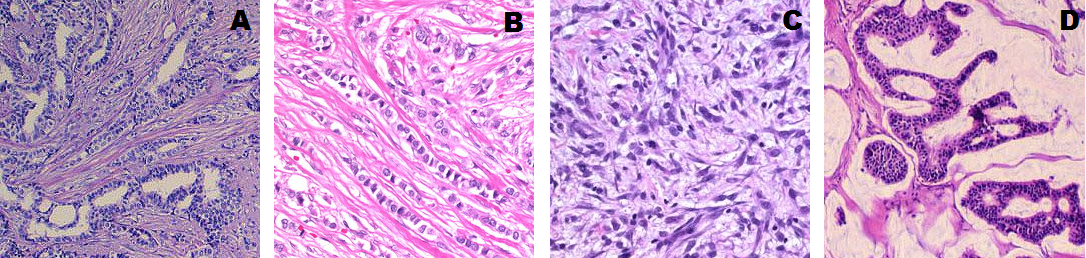
\includegraphics[scale=0.5]{morphology_labelled.png}
            \caption{Breast carcinoma invasive morphologies/histologies. (A) Ductal, (B) Lobular, (C) Metaplastic, (D) Mucinous. Images taken from \cite{Ramnani2016Webpathology.com:Images, Abdelmessieh2016BreastSitu}}
            \label{fig:histology}
            \end{figure} 
    
   Invasive ductal carcinomas and invasive lobular carcinomas have distinct pathological features. Specifically, lobular carcinoma small cells are arranged individually, in single sheet pattern, and they have different molecular and genetic aberrations that distinguish them from ductal carcinomas. The lobular phenotype is determined by dyregulation of cell-cell adhesion, primarily driven by lack of \textit{E}-cadherin protein expression, which is often used as staining marker to tell it apart from the ductal \cite{Ciriello2015ComprehensiveCancer}. Ductal carcinoma has no specific histological characteristics other than invasion through the basement membrane of a breast duct \cite{Weigelt2008RefinementTypes}. 
   
    Metaplastic and mucinous carcinomas are very rare types of breast carcinomas that account for $>1\%$ and $2\%$ of all cases  \cite{Makki2015DiversityRelevance}. 
    Metaplastic breast cancer is a histologically distinct type comprising tumours characterised by a complex admixture of differentiated cells  \cite{Makki2015DiversityRelevance}. It is made up of abnormally looking ductal-origin cells which are thought to have undergone a change in form (\textit{metaplasia}) to become completely different cells that look like soft and connective tissue in the breast. Metaplastic breast cancers are also known to  behave more aggressively than other kinds of breast cancers \cite{schwartz2013metaplastic}. 
    It has been show that $>90\%$ of these cancers lack expression of ER/PR and HER2 (i.e. triple negative), and display a basal-like molecular profile \cite{Weigelt2010a} (more detail in the following sections).


    Mucinous carcinoma is less aggressive than more typical kinds of invasive cancer. The histological hallmark of this carcinoma is the excess of extracellular mucin, which surrounds the cancer cells and becomes part of the tumour \cite{dumitru2015mucinous}.  Mucinous tumours are usually ER/PR positive and HER2 negative, and consistently display a luminal phenotype \cite{Weigelt2010a}. 
    Mucinous tumor cells are less likely to involve the lymph nodes, are more responsive to treatment, and may have a better prognosis than more common types of invasive ductal cancer.

   
   
   
   
   \subsubsection{Receptor status}
            
 
            
    \subsubsection{PAM50 molecular profile}
    % The original studies by Sørlie et al. (Sørlie et al. 2001) classified breast cancer tumours into five intrinsic subtypes with distinct clinical outcomes based on their ‘molecular portrait’: Luminal A, Luminal B, Basal-like, HER2-overexpressed, and Normal-like (Figure 1). The classification was guided by the differences underlying the gene expression patterns that reflect the fundamental differences of the tumours at the molecular level (Sørlie et al. 2003). The observed five subtypes almost perfectly mapped to the previously defined IHC subtypes (Dai et al. 2015), and have been repeated by several other studies with varying number of genes included in the subtypes’ signature. In 2009, Parker et al. (Parker et al. 2009) reported a clinically applicable 50-gene classifier, PAM50, containing mostly hormone receptor and proliferation-related genes. By comparing global gene expression data from microarray and qRT-PCR, a minimized set of 50 genes was identified that could reliably classify each tumour into one of the intrinsic subtypes with 93 accuracy. Over the past 7 years, the PAM50 intrinsic subtypes have shown to provide significant prognostic and predictive information beyond standard clinicopathological parameters (Vidal et al. 2017) (Gnant et al. n.d.). The PAM50 assay is now clinically implemented worldwide using the nCounter platform (Vidal et al. 2017). 

    \subsubsection{Other classifications based on gene expression }

        
    \newpage    
    \subsection{The Cancer Genome Atlas}
        \subsubsection{TCGA goal and setup}
        % The Cancer Genome Atlas (TCGA) network (Anon n.d.), a part of Genomic Data Commons (GDC) from 2016, maintains a public database of clinical and molecular data over 38 different tumour types with hundreds of cases per type, making it the most comprehensive repository of human cancer data (Anon n.d.). Many important marker discovery papers were published with using TCGA data (Colaprico et al. 2016), but opportunities still exist to implement novel methods and test new hypotheses to characterise new biological pathways and diagnostic markers. 
        \subsubsection{TCGA breast cancer dataset}
        % The breast cancer samples available through the TCGA database, among other clinic- and histopathological annotations, are provided with the PAM50 label, allowing for rigorous analysis of the data and room for testing new hypotheses. 

        \subsubsection{TCGA breast cancer dataset previous work}
        
        
        
        
    \subsection{Autophagy}
    % In 2016, a Nobel Prize in Physiology or Medicine was given to Prof Yoshinori Ohsumi (Anon n.d.), a renowned scientist in the autophagy research field, for his success in elucidating the sophisticated machinery of the autophagy pathway. Because of his pioneering work, autophagy is recognized as a fundamental process in cell physiology with major implications for human health and disease. 
    % Autophagy is an evolutionarily conserved lysosomal degradation process that is crucial for adaptation to stress and maintaining cellular homeostasis (Feng et al. 2015). Recent studies have demonstrated association between autophagy and cancer, which implies that autophagy plays an important role in the development, progression, and response of breast cancer cells to chemotherapy and other therapies (Debnath n.d.). 
    
    % Upon starvation or stress conditions, autophagy is induced. Damaged organelles and cytoplasm are sequestered by an expanding phagophore, leading to the formation of double-membrane autophagosome (Feng et al. 2015), as shown in Figure 2. The autophagosome subsequently fuses with the lysosome, followed by the degradation of the sequestered cargo (Yorimitsu and Klionsky 2005). Then, the breakdown products are released back in cytosol through permeases. This allows recycling of the macromolecular constituents as building blocks, to generate energy to maintain cell viability under unfavourable conditions (Feng et al. 2013). 
    % Autophagy is involved in normal aspects of cell development and physiology, and defects in this process are associated with a range of diseases, including cancer. The work of Ohsumi and the colleagues has led to identification several dozens of autophagy-related genes, allowing for targeted research aimed at  understanding of the autophagy mechanisms, with the ultimate goal to manipulate or target them for therapeutic purposes (Feng et al. 2015). 


        \subsubsection{a}
        \subsubsection{b}


        
        
        
        
        
    \subsection{Autophagy in Cancer}
    % The role of autophagy in tumorigenesis and treatment response is complicated and context-dependent, and presumed to differ between stages of cancer progression (Zarzynska and Magdalena 2014). Autophagy’s role in maintaining organelle and protein turnover allows cells to restrain damage, including genome instability and inflammation, thereby limiting initiation and progression of cancer at early stages. However, once tumour develops, the cancer cells are able to utilize autophagy for their own cytoprotection (Zarzynska and Magdalena 2014). Autophagy is believed to promote cancer by allowing cells to survive under conditions of metabolic and genotoxic stress (Mathew and White n.d.). Unfavourable conditions such as hypoxia and acidity in tumour environment as well as the effects of chemo- and radiotherapy cause cells to experience stress and nutrient deprivation (Bailey et al. n.d.). Induction of autophagy within these cells allows them to survive the drastic conditions. This kind of mechanism had been referred to as “what doesn’t kill you, makes you stronger” by researchers in the field (Mathew and White n.d.).
        \subsubsection{a}
        \subsubsection{b}
        
        
        


\section{Thesis objectives}
% The role of autophagy in tumorigenesis and treatment response is complicated and context-dependent, and presumed to differ between stages of cancer progression (Zarzynska and Magdalena 2014). Autophagy’s role in maintaining organelle and protein turnover allows cells to restrain damage, including genome instability and inflammation, thereby limiting initiation and progression of cancer at early stages. However, once tumour develops, the cancer cells are able to utilize autophagy for their own cytoprotection (Zarzynska and Magdalena 2014). Autophagy is believed to promote cancer by allowing cells to survive under conditions of metabolic and genotoxic stress (Mathew and White n.d.). Unfavourable conditions such as hypoxia and acidity in tumour environment as well as the effects of chemo- and radiotherapy cause cells to experience stress and nutrient deprivation (Bailey et al. n.d.). Induction of autophagy within these cells allows them to survive the drastic conditions. This kind of mechanism had been referred to as “what doesn’t kill you, makes you stronger” by researchers in the field (Mathew and White n.d.).

